\documentclass[10pt,journal]{IEEEtran}

\usepackage{cite}
\usepackage{amsmath,amssymb,amsfonts,amsthm,mathtools}
\usepackage{booktabs,multirow,array}
\usepackage{graphicx}
\usepackage{url}
\usepackage{xcolor}
\usepackage{enumitem}
\usepackage{microtype}
\usepackage{threeparttable}
\usepackage{makecell}
\usepackage{tabularx}
\usepackage{algorithm}
\usepackage[noend]{algpseudocode}
\usepackage{hyperref}
\hypersetup{hidelinks}

\graphicspath{{figures/}{./}}

\newcolumntype{Y}{>{\centering\arraybackslash}X}
\newcommand{\best}[1]{\textbf{#1}}
\newcommand{\localonly}{local-only}
\newcommand{\statsonly}{stats-only}
\newcommand{\statstransfer}{stats-transfer}
\newcommand{\prototransfer}{prototype-transfer}
\newcommand{\R}{\mathbb{R}}
\newcommand{\E}{\mathbb{E}}
\newcommand{\norm}[1]{\left\lVert #1 \right\rVert}
\newcommand{\inner}[2]{\left\langle #1, #2 \right\rangle}
\newcommand{\tr}{\mathrm{tr}}
\newcommand{\deficit}{\boldsymbol{\delta}}
\newcommand{\nclients}{K_{\mathrm{cl}}}

\newtheorem{proposition}{Proposition}
\newtheorem{remark}{Remark}

\title{PALM-FL: Low-Payload Client-Summary Coordination and Resource-Aware Scheduling for Heterogeneous Mobile Federated Learning}

\author{Author Name(s) Omitted for Review}

\markboth{}{PALM-FL}

\begin{document}
\maketitle

\begin{abstract}
Model heterogeneity is a practical obstacle to federated learning on mobile devices. In realistic deployments, clients differ in architecture, compute capability, memory budget, battery state, and link quality, making weight sharing through a single global model restrictive. This paper presents PALM-FL, a heterogeneous federated learning framework that keeps client architectures local and exchanges only compact clipped-and-noised client summaries. Each selected client uploads class-wise counts, latent means, and diagonal variances, and the server uses the resulting summary memory for budget-aware client selection rather than model aggregation. The zero-downlink \statsonly{} path remains architecture-agnostic at the server, while a masked \statstransfer{} path uses the same compact memory for prototype-contrastive local regularization. The evaluation uses independent Dirichlet repartitions and trace-derived mobile profiles built from 49,760 public 4G, 5G, and WiFi bandwidth measurements. On MNIST, finite-noise random transfer reaches $56.11\pm3.99\%$ accuracy over three independent partitions, compared with $52.12\pm4.21\%$ for \localonly{} and $51.59\pm4.74\%$ for \statsonly{}. On a trace-calibrated CIFAR-10 seed-42 case study, random transfer reaches $29.47\%$ accuracy, while mobile-aware transfer remains close to local/statistics baselines. Homogeneous FedAvg remains more accurate but requires a common architecture and full-model exchange. These results support PALM-FL as a low-payload, architecture-flexible coordination mechanism whose \statsonly{} mode preserves local performance and whose transfer mode can help when participation coverage is broad enough.
\end{abstract}

\begin{IEEEkeywords}
Federated learning, model heterogeneity, mobile computing, privacy accounting, communication efficiency, client scheduling.
\end{IEEEkeywords}

\section{Introduction}
\IEEEPARstart{F}{ederated} learning allows multiple clients to train models collaboratively without centralizing raw data. Most federated learning methods, however, still assume that participating clients can train variants of a single shared model \cite{fedavg,fedprox,scaffold}. This assumption is increasingly difficult to justify in mobile systems. Smartphones, wearables, and embedded edge devices differ substantially in compute capability, memory budget, battery state, accelerator support, and link quality \cite{pfeiffer,nguyen}. In practice, many devices can host only lightweight client-specific architectures, while others depend on proprietary or hardware-tuned models that cannot be exposed or modified.

Model-heterogeneous federated learning has therefore become an important problem. Existing approaches address it in several ways. Supernet and submodel methods allow clients to train different-capacity models, but they still confine them to a common architecture family \cite{fjord,heterofl,depthfl,nefl}. Distillation-based methods permit broader heterogeneity, but often rely on proxy data, repeated logit exchange, or auxiliary public datasets \cite{avgkd,feddf,fccl,fedmd,fedgh,pfedhr}. Representation-sharing methods reduce the mismatch by introducing a common feature module, although they weaken full architectural autonomy \cite{lgfedavg,fml,fedclassavg,mori}.

GEFL introduced generative transfer for heterogeneous federated learning, and GEFL-F reduced its cost by moving from image synthesis to feature synthesis through a shared extractor \cite{gefl}. Even so, both approaches still require the exchange of global generative state. In mobile settings, that design raises two related questions. First, how should cross-client information be shared when communication, latency, energy, and privacy are all constrained? Second, how much of the server state must be coupled to client architectures?

This paper addresses these questions through PALM-FL. The central idea is to move the main server-side coordination path away from generator broadcast and toward clipped-and-noised client-summary release. Each client keeps its encoder, adapter, and prediction head local. Instead of uploading parameters or downloading synthetic features, the client computes compact class-wise counts and latent summaries, clips and perturbs them, and sends only the sanitized summaries to the server. The server maintains a global summary memory and uses it to guide budget-aware client selection under explicit uplink, downlink, energy, and round-time constraints. The default operating mode therefore requires no model download and no architecture alignment across clients.

The contributions of this work are as follows.
\begin{enumerate}[leftmargin=1.25em]
    \item We propose PALM-FL, a heterogeneous mobile federated learning framework in which the server coordinates training from compact clipped client summaries rather than architecture-specific parameter alignment.
    \item We develop a clipped-and-noised summary-release mechanism for class-wise counts, latent means, and diagonal variances that supports zero-downlink operation in the main training path.
    \item We introduce a resource-aware client scheduler that balances data utility, class coverage, staleness, battery state, communication, and time under explicit mobile budgets.
    \item We evaluate the method with independent Dirichlet repartitions on MNIST and trace-derived mobile profiles built from public 4G, 5G, and WiFi bandwidth measurements.
    \item We evaluate heterogeneous MNIST and CIFAR-10 clients and show that \statsonly{} closely tracks, rather than substantially improves over, \localonly{} while maintaining zero downlink and small uplink.
    \item We include a masked prototype-contrastive \statstransfer{} variant and show that it improves MNIST accuracy under random participation, while mobile-aware CIFAR-10 transfer remains a low-payload but scheduler-sensitive operating point.
    \item We include homogeneous FedAvg, FedProto-style, and FedMD-style references that expose the trade-off among accuracy, communication, architecture autonomy, proxy data, and prototype exchange.
    \item We report per-architecture fairness summaries and show that scheduler choice defines a real trade-off: random participation improves utility, while mobile-aware selection controls operating cost.
\end{enumerate}

\begin{figure*}[t]
    \centering
    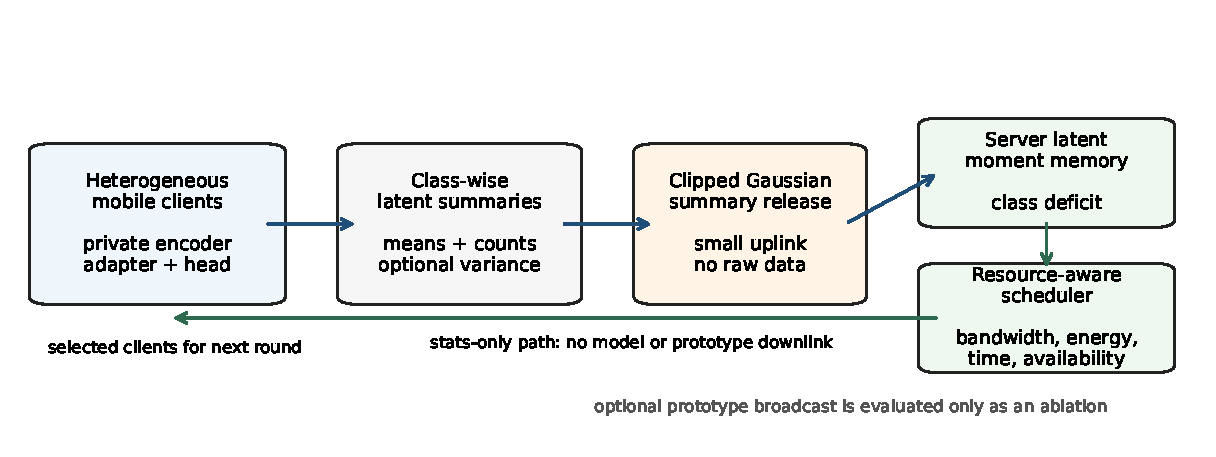
\includegraphics[width=0.96\textwidth]{fig1_tmc_overview.pdf}
    \caption{Overview of PALM-FL. Each client keeps its encoder, adapter, and prediction head private, extracts compact class-wise latent moments, clips and perturbs them before upload, and is selected by a resource-aware scheduler subject to communication, energy, and round-time budgets. In the default \statsonly{} mode, the server uses the latent memory only for scheduling and does not broadcast models or prototypes back to the clients.}
    \label{fig:overview}
\end{figure*}

\section{Related Work}
\subsection{Homogeneous federated learning and mobile FL systems}
FedAvg remains the standard baseline for homogeneous federated learning, while FedProx, SCAFFOLD, and adaptive local aggregation variants improve robustness under statistical and systems heterogeneity \cite{fedavg,fedprox,scaffold,fedala}. Surveys on constrained and IoT federated learning emphasize that realistic edge deployments must manage client-side limitations in computation, memory, energy, and network bandwidth rather than optimize only for accuracy \cite{pfeiffer,nguyen}. PALM-FL follows that systems view directly.

\subsection{Model-heterogeneous federated learning}
The heterogeneous-FL literature can be grouped into several families. A first family scales a shared supernet or global architecture into client-specific submodels, as in FjORD, HeteroFL, DepthFL, and NeFL \cite{fjord,heterofl,depthfl,nefl}. These methods are effective when clients remain within the same architecture family, but they do not provide full architectural autonomy. A second line of work addresses heterogeneity through distillation, ensembling, or proxy-data transfer, including AvgKD, FedDF, FCCL, FedMD, FedGH, and pFedHR \cite{avgkd,feddf,fccl,fedmd,fedgh,pfedhr}. Prototype-sharing methods such as FedProto exchange class prototypes instead of gradients or complete weights \cite{fedproto}. These methods permit broader heterogeneity, but often depend on proxy data, repeated logit exchange, auxiliary public datasets, or unmasked class prototypes. A third family shares a representation module or auxiliary model, as in LG-FedAvg, federated mutual learning, FedClassAvg, and continual horizontal FL for heterogeneous data \cite{lgfedavg,fml,fedclassavg,mori}. These approaches reduce part of the mismatch, but they still impose a partially shared representation.

\subsection{Generator-centered transfer and privacy}
Generator-centered FL has been explored through federated GANs, conditional feature generators, and data-free distillation \cite{fedgan,fedcg,datafreekd,finetunekd}. GEFL is the closest precursor to this paper. It uses a federated generator to transfer global knowledge across clients with different models, and GEFL-F reduces the cost of that idea by shifting from image generation to feature generation through a shared extractor \cite{gefl}. The base paper also highlights the remaining issues: privacy leakage through memorization, performance degradation as client count grows, and the resource overhead of the shared generative state \cite{gefl}. Representation release can also be vulnerable to inversion-style attacks \cite{zeiler,mahendran,dosovitskiy}. PALM-FL addresses the same problem family by using compact latent moments rather than generator broadcast as the main exchange primitive.

Table~\ref{tab:prior_compare} summarizes representative methods discussed in the base paper and related literature. PALM-FL is the only row that combines client-specific heterogeneous architectures, no shared extractor, zero-downlink operation in the main path, and explicit budget-aware scheduling.

\begin{table*}[t]
\centering
\caption{Design-space comparison with representative heterogeneous federated learning methods. ``Partial'' indicates that clients can differ in capacity or head structure but still remain within a shared supernet, extractor, or representation family. PALM-FL still assumes a shared latent dimension through private adapters in the summary-release path.}
\label{tab:prior_compare}
\begin{threeparttable}
\setlength{\tabcolsep}{4pt}
\scriptsize
\begin{tabularx}{\textwidth}{lYYYYYY}
\toprule
Method family & Client-specific arch. & Proxy data & Shared module & Default payload & Zero-downlink & Mobile-aware \\
\midrule
Homogeneous FL \cite{fedavg,fedprox,fedala} & No & No & Yes & weights & No & No \\
Submodel / supernet FL \cite{fjord,heterofl,depthfl,nefl} & Partial & No & Yes & submodel & No & No \\
Proxy-data distillation FL \cite{avgkd,feddf,fccl,fedmd,fedgh,pfedhr} & Yes & Often yes & No & logits / models & No & No \\
Representation-sharing FL \cite{lgfedavg,fml,fedclassavg,mori} & Partial & No & Yes & representation weights & No & No \\
GEFL \cite{gefl} & Yes & No & No & generator & No & No \\
GEFL-F \cite{gefl} & Partial & No & Yes & feature generator & No & No \\
PALM-FL & \best{Yes} & \best{No} & \best{No} & \best{summaries} & \best{Yes} & \best{Yes} \\
\bottomrule
\end{tabularx}
\end{threeparttable}
\end{table*}

\section{System Model and Objective}
We consider a cross-device federated learning system with client set $\mathcal{K} = \{1,\dots,\nclients\}$. Client $k$ stores a private dataset
\begin{equation}
\mathcal{D}_k = \{(x_i,y_i)\}_{i=1}^{N_k}, \qquad y_i \in \{1,\dots,C\},
\end{equation}
and uses a private model
\begin{equation}
f_k(x;\theta_k) = H_k(A_k(E_k(x))),
\label{eq:model}
\end{equation}
where $E_k$ is a private encoder, $A_k$ is a private latent adapter, and $H_k$ is a private prediction head. The latent representation is
\begin{equation}
z_i^{(k)} = A_k(E_k(x_i)) \in \R^d,
\end{equation}
where the latent dimension $d$ is shared, but the client backbones and heads may differ completely.

Each client is associated with a device profile
\begin{equation}
\psi_k = (b_k, c_k, e_k, a_k),
\end{equation}
where $b_k$ is available bandwidth, $c_k$ is normalized compute throughput, $e_k$ is remaining battery energy, and $a_k \in [0,1]$ is an availability probability. In round $t$, the server selects a subset $\mathcal{S}_t \subseteq \mathcal{K}$ subject to a maximum participation size $M$ and the system budgets
\begin{align}
\sum_{k\in\mathcal{S}_t} U_k^t &\le B_{\text{up}}, \\
\sum_{k\in\mathcal{S}_t} D_k^t &\le B_{\text{down}}, \\
\sum_{k\in\mathcal{S}_t} E_k^t &\le B_{\text{eng}}, \\
\max_{k\in\mathcal{S}_t} T_k^t &\le B_{\text{time}},
\end{align}
where $U_k^t$, $D_k^t$, $E_k^t$, and $T_k^t$ denote the predicted uplink, downlink, energy, and round-time cost for client $k$ in round $t$.

The overall objective is to coordinate local training and scheduling under these constraints while limiting information exposure from the released summaries:
\begin{align}
\min_{\{\theta_k\},\pi} \quad & \sum_{t=1}^{T}\sum_{k\in\mathcal{S}_t}\mathcal{L}_k(\theta_k;\mathcal{D}_k)
\label{eq:global_problem}\\
\text{s.t.}\quad & \mathcal{S}_t = \pi(\mathcal{H}_t,\mathcal{M}_t), \quad |\mathcal{S}_t| \le M,
\nonumber\\
& \text{the mobile budgets hold in every round}.
\nonumber
\end{align}
Here $\mathcal{H}_t$ is the server-side state and $\mathcal{M}_t$ is the collection of clipped-and-noised client summaries available at round $t$.

\section{PALM-FL Method}
\subsection{Client-side summary extraction}
Each selected client computes class-wise counts and latent moments from its local minibatches. For class $c$, define
\begin{align}
n_{k,c} &= \sum_{(x,y)\in\mathcal{D}_k}\mathbb{I}[y=c], \\
\mu_{k,c} &= \frac{1}{\max(n_{k,c},1)}
\sum_{(x,y)\in\mathcal{D}_k} z(x)\,\mathbb{I}[y=c], \\
v_{k,c} &= \frac{1}{\max(n_{k,c},1)}
\sum_{(x,y)\in\mathcal{D}_k} z(x)\odot z(x)\,\mathbb{I}[y=c]
\nonumber\\
&\quad -\mu_{k,c}\odot\mu_{k,c},
\end{align}
where $z(x)=A_k(E_k(x))$ and $\odot$ denotes elementwise multiplication. The implementation releases the class mean, diagonal variance, noisy count, and a count-derived availability mask. The \statsonly{} mode uses these summaries only on the server side; it does not broadcast prototypes or models to clients. In this default path, the class-deficit term is count-driven, so the current results should not be interpreted as isolating the marginal value of latent means over clipped-and-noised class-count balancing.

This choice is practical for mobile devices. The uploaded state scales with the latent dimension $d$ and the class count $C$, and is independent of the parameter count of the client model. The server therefore needs no architecture-specific merger, no backbone alignment, and no global decoder.

\subsection{Clipped-and-noised moment release}
Before transmission, PALM-FL clips the client summaries and perturbs them with Gaussian noise. Let $M_k=[\mu_{k,1};\ldots;\mu_{k,C}]$ and $V_k=[v_{k,1};\ldots;v_{k,C}]$ stack the class-wise mean and diagonal-variance vectors, and let $\mathbf{n}_k=(n_{k,1},\ldots,n_{k,C})$. The privacy unit in the current implementation is the released client-summary object, not an individual raw training example: two summary inputs are treated as adjacent when their clipped released statistic differs by at most the stated $\ell_2$ bound. With clipping thresholds $S_{\mu}$, $S_v$, and $S_n$, the released summaries are
\begin{align}
\widehat{M}_k &= \operatorname{clip}_2(M_k,S_{\mu}) + \Xi_k, \\
\widehat{V}_k &= \operatorname{clip}_2(V_k,S_v) + \Psi_k, \\
\widehat{\mathbf{n}}_k &=
\operatorname{clip}_2(\max(\mathbf{n}_k,0),S_n) + \boldsymbol{\zeta}_k,
\end{align}
where
\begin{align}
\operatorname{vec}(\Xi_k)&\sim\mathcal{N}(0,\sigma^2 S_{\mu}^2 I),\\
\operatorname{vec}(\Psi_k)&\sim\mathcal{N}(0,\sigma^2 S_v^2 I),\\
\boldsymbol{\zeta}_k&\sim\mathcal{N}(0,\sigma^2 S_n^2 I).
\end{align}
The rows of $\widehat{M}_k$ and $\widehat{V}_k$ define $\widehat{\mu}_{k,c}$ and $\widehat{v}_{k,c}$, and the entries of $\widehat{\mathbf{n}}_k$ define $\widehat{n}_{k,c}$. Released counts are truncated to be nonnegative, and the mask is computed by thresholding the noisy count. In our implementation, privacy is accumulated over participating rounds with a participation-counted zCDP-style accountant \cite{abadi,zcdp}. The reported privacy values should be interpreted as accounting values for clipped client-summary release; the learned latent summaries are not accompanied by a sample-level sensitivity proof, and stronger sample-level certification would require per-example clipping and accounting.

\subsection{Server-side latent memory and deficit estimation}
Let $\beta\in[0,1)$ denote the server exponential moving average factor. For each class $c$, the server ignores client payloads whose count-derived mask is false and then forms the round-level sufficient statistics
\begin{align}
\widetilde{N}_c^{(t)} &=
\sum_{k\in\mathcal{S}_t}\widehat{n}_{k,c}, \\
\widetilde{\mu}_c^{(t)} &=
\frac{\sum_{k\in\mathcal{S}_t}\widehat{n}_{k,c}\widehat{\mu}_{k,c}}
{\max\!\left(\widetilde{N}_c^{(t)},\epsilon\right)},\\
\widetilde{q}_c^{(t)} &=
\frac{\sum_{k\in\mathcal{S}_t}\widehat{n}_{k,c}
\left(\widehat{v}_{k,c}+\widehat{\mu}_{k,c}\odot\widehat{\mu}_{k,c}\right)}
{\max\!\left(\widetilde{N}_c^{(t)},\epsilon\right)},\\
\widetilde{v}_c^{(t)} &= \max\!\left(\widetilde{q}_c^{(t)}
-\widetilde{\mu}_c^{(t)}\odot\widetilde{\mu}_c^{(t)}, v_{\min}\right).
\end{align}
It then updates the class count, prototype mean, and diagonal variance with exponential memory, matching the implemented aggregator:
\begin{align}
N_c^{(t)} &= \beta N_c^{(t-1)}
+ (1-\beta)\widetilde{N}_c^{(t)}, \\
\bar{\mu}_c^{(t)} &= \beta\bar{\mu}_c^{(t-1)}
+ (1-\beta)\widetilde{\mu}_c^{(t)},\\
\bar{v}_c^{(t)} &= \beta\bar{v}_c^{(t-1)}
+ (1-\beta)\widetilde{v}_c^{(t)}.
\end{align}
Previously unseen classes are initialized from the first observed $\widetilde{\mu}_c^{(t)}$ rather than from the zero vector.
The global class deficit vector is
\begin{equation}
\deficit_c^{(t)} =
\frac{\max_j N_j^{(t)} - N_c^{(t)}}
{\sum_{m=1}^{C}\left(\max_j N_j^{(t)} - N_m^{(t)}\right)+\epsilon},
\label{eq:deficit}
\end{equation}
which assigns larger weight to underrepresented classes. In \statsonly{}, the server does not broadcast $\bar{\mu}_c^{(t)}$ to clients. Instead, the deficit vector $\deficit^{(t)}$ is consumed only by the scheduler, which avoids additional downlink and keeps the main learning path architecture-agnostic. This also scopes the role of the latent means: in \statsonly{}, class counts drive the deficit term, while the latent means and variances maintain the server memory used by the optional transfer path.

\subsection{Resource-aware scheduling}
For each candidate client, the server estimates communication and compute cost from device metadata. The predicted time and energy are modeled as
\begin{align}
T_k^t &= \frac{8U_k^t}{b_k} + \frac{8D_k^t}{b_k} + \alpha_T\frac{L_kP_k}{c_k}, \\
E_k^t &= \alpha_U(U_k^t + D_k^t) + \alpha_E L_kP_k,
\end{align}
where $P_k$ is the model size in MB-equivalent parameters, $L_k$ is the estimated number of local steps, and $\alpha_T$, $\alpha_U$, and $\alpha_E$ map bandwidth and compute to time and energy.

The scheduler assigns utility to client $k$ in round $t$ using data availability, estimated label diversity, staleness, battery state, recent loss, and deficit coverage:
\begin{align}
u_k^t &= w_d s_k + w_{\ell}\ell_k + w_r r_k + w_b q_k + w_v \nu_k
\nonumber\\
&\quad + w_c\,\inner{\mathbf{1}[\widehat{h}_k>0]}{\deficit^{(t)}}
- \lambda_u\frac{U_k^t}{B_{\text{up}}}
- \lambda_d\frac{D_k^t}{B_{\text{down}}}
\nonumber\\
&\quad
- \lambda_e\frac{E_k^t}{B_{\text{eng}}} 
- \lambda_t\frac{T_k^t}{B_{\text{time}}},
\label{eq:utility}
\end{align}
where $s_k$ is a normalized sample-count score, $\ell_k$ is a normalized recent-loss score, $r_k$ is a staleness score, $q_k$ is remaining battery fraction, $\nu_k$ is an estimated label-diversity score, and $\widehat{h}_k\in\R^C$ is the most recent clipped-and-noised client count vector available to the server. The scheduler does not require raw label histograms before selection; clients with no prior accepted summary use a zero class-coverage vector until they participate. The selected client set is obtained from
\begin{align}
\max_{\mathcal{S}\subseteq\mathcal{K}} \quad & \sum_{k\in\mathcal{S}} u_k^t \\
\text{s.t.}\quad
& \sum_{k\in\mathcal{S}} U_k^t \le B_{\text{up}}, \quad
\sum_{k\in\mathcal{S}} D_k^t \le B_{\text{down}}, \nonumber\\
& \sum_{k\in\mathcal{S}} E_k^t \le B_{\text{eng}}, \quad
\max_{k\in\mathcal{S}} T_k^t \le B_{\text{time}}, \quad
|\mathcal{S}| \le M. \nonumber
\end{align}
In our implementation, this problem is solved with a ratio-greedy selection rule that orders clients by utility normalized by budget consumption.

\subsection{Local optimization}
The default local objective combines classification loss with a covariance regularizer on the latent representation:
\begin{equation}
\mathcal{L}_k = \E_{(x,y)\sim\mathcal{D}_k}\big[\mathrm{CE}(f_k(x),y)\big]
+ \lambda_{\mathrm{cov}}\Omega(z),
\label{eq:local_loss}
\end{equation}
where $\Omega(z)$ penalizes deviations of the latent covariance from the identity matrix. If $Z\in\R^{B\times d}$ is the minibatch latent matrix, then
\begin{equation}
\Omega(z)=
\frac{1}{d}\sum_{j=1}^{d}(\Sigma_{jj}-1)^2
+\frac{1}{d(d-1)}\sum_{i\neq j}\Sigma_{ij}^2,
\end{equation}
with $\Sigma=\frac{1}{B}(\widetilde{Z}^{\top}\widetilde{Z})$ and $\widetilde{Z}$ the standardized latent matrix. This regularizer stabilizes the latent space while remaining fully local.

\subsection{Masked prototype-contrastive transfer}
PALM-FL also supports a \statstransfer{} variant in which the server broadcasts a compact masked prototype package derived from the latent memory. The package contains available class prototypes, diagonal variances, class counts, and class priors. A class is marked available only when its sanitized count exceeds a configurable threshold, which prevents absent or noise-dominated classes from polluting the prototype bank.

When a prototype package is available after warm-up, selected clients add two lightweight local transfer terms. The first aligns real-batch latents with their own available class prototype:
\begin{equation}
\mathcal{L}_{\mathrm{align}} =
\E_{(x,y)}\left[\mathbf{1}[m_y=1]
\left\lVert
\frac{z(x)}{\lVert z(x)\rVert_2}
-
\frac{\bar{\mu}_y}{\lVert\bar{\mu}_y\rVert_2}
\right\rVert_2^2
\right],
\end{equation}
where $m_y$ is the server mask for class $y$. The second treats the available prototypes as class anchors. Define
\begin{equation}
s_c(x)=\frac{\langle \mathrm{norm}(z(x)),\mathrm{norm}(\bar{\mu}_c)\rangle}{\tau}.
\end{equation}
The prototype-contrastive cross-entropy is
\begin{equation}
\mathcal{L}_{\mathrm{pCE}} =
\E_{(x,y):m_y=1}
\left[
-\log
\frac{\exp(s_y(x))}
{\sum_{c:m_c=1}\exp(s_c(x))}
\right].
\end{equation}
The resulting local objective is
\begin{equation}
\mathcal{L}_k^{\mathrm{transfer}} =
\mathcal{L}_k
+ \lambda_a\mathcal{L}_{\mathrm{align}}
+ \lambda_p\mathcal{L}_{\mathrm{pCE}}.
\end{equation}
This differs from unmasked prototype-broadcast ablations: unavailable classes are explicitly masked and the contrastive term uses other available global prototypes as negatives. It adds a small downlink proportional to $Cd$, but still avoids model, gradient, generator, or decoder broadcast.

\begin{algorithm}[t]
\caption{PALM-FL round with optional masked \statstransfer{}}
\label{alg:palmfl}
\begin{algorithmic}[1]
\Require client set $\mathcal{K}$, latent memory $(\bar{\mu}^{(t-1)},N^{(t-1)})$, budgets $(B_{\text{up}},B_{\text{down}},B_{\text{eng}},B_{\text{time}})$
\State compute deficit vector from \eqref{eq:deficit}
\State estimate $(U_k^t,D_k^t,E_k^t,T_k^t)$ for all eligible clients
\State select $\mathcal{S}_t$ with the budget-aware scheduler
\ForAll{$k\in\mathcal{S}_t$ in parallel}
    \State train the private model with loss \eqref{eq:local_loss}
    \State compute $(n_{k,c},\mu_{k,c},v_{k,c})$ for all classes $c$
    \State privatize $(n_{k,c},\mu_{k,c},v_{k,c})$ with clipped Gaussian release
    \State upload $(\widehat{n}_{k,c},\widehat{\mu}_{k,c},\widehat{v}_{k,c},m_{k,c})$
\EndFor
\State aggregate uploaded moments into $(\bar{\mu}^{(t)},\bar{v}^{(t)},N^{(t)})$ and class mask $m^{(t)}$
\If{\statstransfer{} is enabled and warm-up has ended}
    \State export masked prototype package to selected clients in the next round
\EndIf
\State update the scheduler state with observed loss, participation, and device cost
\end{algorithmic}
\end{algorithm}

\begin{algorithm}[t]
\caption{Budget-aware client selection}
\label{alg:scheduler}
\begin{algorithmic}[1]
\Require candidate clients $\mathcal{A}_t$, utility scores $u_k^t$, per-client costs $(U_k^t,D_k^t,E_k^t,T_k^t)$, maximum size $M$
\State sort candidates by utility normalized by budget consumption
\State initialize $\mathcal{S}_t\leftarrow\emptyset$
\ForAll{$k$ in sorted order}
    \If{$|\mathcal{S}_t| = M$}
        \State \textbf{break}
    \EndIf
    \If{adding client $k$ violates an uplink, downlink, energy, or time budget}
        \State \textbf{continue}
    \EndIf
    \State add $k$ to $\mathcal{S}_t$
\EndFor
\If{$\mathcal{S}_t=\emptyset$}
    \State return the best single feasible client
\EndIf
\State \Return $\mathcal{S}_t$
\end{algorithmic}
\end{algorithm}

\subsection{Analysis}
\begin{proposition}[Communication complexity]
If class-wise means, diagonal variances, counts, and masks are uploaded, then the per-round uplink of client $k$ in \statsonly{} is $\mathcal{O}(2Cd+C)$ scalars and does not depend on the parameter count of $f_k$.
\end{proposition}
\begin{IEEEproof}
The uploaded state contains one $d$-dimensional mean vector, one $d$-dimensional diagonal variance vector, one scalar count, and one mask bit per class, which requires $2Cd+\mathcal{O}(C)$ scalars. This is $\mathcal{O}(Cd)$ for fixed moment order and class count.
\end{IEEEproof}

\begin{proposition}[Architecture-agnostic server state]
The server-side state of PALM-FL depends only on latent dimension $d$, class count $C$, clipped count summaries, and scalar resource metadata. It does not require layer-wise parameter aggregation, weight matching, or architecture-specific adapters.
\end{proposition}
\begin{IEEEproof}
The server receives only sanitized moments and device metadata. The latent-memory update and the scheduler operate on these quantities only; no step depends on the internal parameterization of $E_k$, $A_k$, or $H_k$.
\end{IEEEproof}

\begin{proposition}[Client-summary Gaussian accounting]
Suppose each released client-summary statistic is clipped to its stated summary-level sensitivity and perturbed with Gaussian noise calibrated to that sensitivity. Then each statistic satisfies the standard Gaussian-mechanism guarantee for the clipped summary under the summary-level adjacency relation described above. For a client that participates in $R_k$ rounds with $r$ Gaussian releases per round, the accountant used here tracks
\begin{equation}
\rho_k = \frac{R_k r}{2\sigma^2},\qquad
\varepsilon_k(\delta)=\rho_k+2\sqrt{\rho_k\log(1/\delta)}.
\end{equation}
\end{proposition}

\begin{remark}
The experiments reported here use a participation-counted zCDP-style accountant. This is sufficient for comparing operating modes under the same release mechanism, but it is not a complete sample-level privacy certificate. The reported $\varepsilon$ values are also large, so the mechanism should be interpreted as clipped-and-noised summary release with accounting rather than strong end-to-end differential privacy.
\end{remark}

\begin{table}[t]
\centering
\caption{Privacy-accounting parameters used in the finite-noise summary-release rows. ``N/A'' means the method is not accounted under PALM-FL's clipped summary-release mechanism.}
\label{tab:privacy_accounting}
\scriptsize
\setlength{\tabcolsep}{3pt}
\begin{tabularx}{\columnwidth}{lXXl}
\toprule
Mode & Released objects & Accounting unit & Interpretation \\
\midrule
\localonly{} & none & N/A & no summary-release accountant \\
\statsonly{} & counts, means, variances; $S_{\mu}=S_v=4$, $S_n=200$, $\sigma=0.5$, $\delta=10^{-5}$ & client summary & high $\varepsilon$; not sample-level DP \\
\statstransfer{} & same upload plus masked prototype package downlink & client summary & high $\varepsilon$; not sample-level DP \\
FedAvg & model weights & N/A & not private by this accountant \\
FedMD-style & proxy logits & N/A & not private by this accountant \\
\bottomrule
\end{tabularx}
\end{table}

\section{Experimental Setup}
\subsection{Datasets, clients, and models}
We evaluate PALM-FL on MNIST and CIFAR-10 \cite{mnist,cifar10} under heterogeneous cross-device partitioning. Both datasets are divided across ten clients using a Dirichlet partition with $\alpha=0.3$, which creates strong label skew while preserving client diversity. Each client uses one of four lightweight architectures: \texttt{small\_cnn}, \texttt{wide\_cnn}, \texttt{tiny\_resnet}, or \texttt{tiny\_mobilenet}. All models on a dataset share only the adapter output dimension: $d=48$ for MNIST and $d=64$ for CIFAR-10.

\subsection{Trace-derived mobile profiles}
To move beyond a purely synthetic mobile profile, we derive the bandwidth component of the scheduler profiles from the public Mobile Access Bandwidth in Practice release \cite{mobilebandwidth}. The release contains anonymized representative samples from 49,760 Android bandwidth tests across 4G, 5G, WiFi~4, WiFi~5, and WiFi~6. We construct a deterministic ten-client profile file by selecting technology-stratified bandwidth quantiles from the released CSV files. The resulting trace profiles span 1.2--681.2 Mbps in this run and are used by PALM-FL, FedAvg, FedProto-style, and FedMD-style experiments through the same scheduler interface. Compute throughput, battery capacity, recharge, and per-step energy remain model parameters because the bandwidth trace does not include direct model-training energy measurements. Thus, the reported time and energy values are trace-calibrated operating estimates, not phone power-meter measurements.

\subsection{Training, baselines, and metrics}
MNIST uses 15 rounds with 3 warm-up rounds and a 0.4 participation rate. The MNIST rows report mean and sample standard deviation over seeds 42, 43, and 44, with the client partition seed and architecture seed both varied with the training seed. CIFAR-10 uses 20 rounds, 4 warm-up rounds, evaluation every five rounds, and a full final evaluation. Because full trace-calibrated CIFAR-10 independent reruns are substantially more expensive in this implementation, the CIFAR-10 rows in Table~\ref{tab:main_results} are reported as a completed seed-42 trace case study; fixed-split three-seed CIFAR artifacts are retained in the reproducibility bundle but are not used for the independent-split claim.

We compare \localonly{}, \statsonly{}, mobile-scheduled \statstransfer{}, and random-scheduled \statstransfer{}. We also include three references. Homogeneous FedAvg uses a shared \texttt{small\_cnn}; FedProto-style keeps heterogeneous clients but disables PALM stat-head and prototype-contrastive terms; FedMD-style uses a public proxy split and exchanges averaged proxy logits. We report accuracy, macro-F1, uplink, downlink, trace-calibrated predicted round time, predicted energy, and privacy loss from the participation-counted zCDP-style accountant where that accountant is part of the method. Rows without this mechanism are marked as not DP-accounted rather than assigned an $\varepsilon$ value. Finite-noise summary-release rows use $S_{\mu}=S_v=4.0$, $S_n=200$, $\delta=10^{-5}$, and $\sigma=0.5$. Accuracy is averaged over client-local models under a low-round, low-participation, non-IID protocol, so the MNIST values are not intended to match fully centralized or long-horizon MNIST training.

\subsection{Implementation and reproducibility}
All experiments are executed from the same implementation tree and stored as completed run artifacts. The package includes the trace-profile builder, independent-split experiment driver, FedMD-style baseline, aggregation scripts, curated CSV files, regenerated figures, and per-client final metrics for fairness analysis. The public artifact repository is available at \url{https://github.com/Devchandrasen/PALM-FL-TMC-Artifact}.

\section{Results}
\subsection{Operating-mode comparison}
Table~\ref{tab:main_results} presents the operating-mode comparison. On MNIST, random-scheduled \statstransfer{} reaches $56.11\pm3.99\%$ accuracy over three independent partitions, compared with $52.12\pm4.21\%$ for \localonly{} and $51.59\pm4.74\%$ for \statsonly{}. Mobile-scheduled transfer remains close to \statsonly{}, which means the mobile policy is better interpreted as a cost-control policy than as an accuracy maximizer. On the CIFAR-10 seed-42 trace case study, random transfer reaches $29.47\%$ accuracy, while mobile transfer remains near the local/statistics baselines. This confirms a consistent scheduler-sensitive pattern without overstating mobile transfer as a universal accuracy improvement.

\begin{figure*}[t]
    \centering
    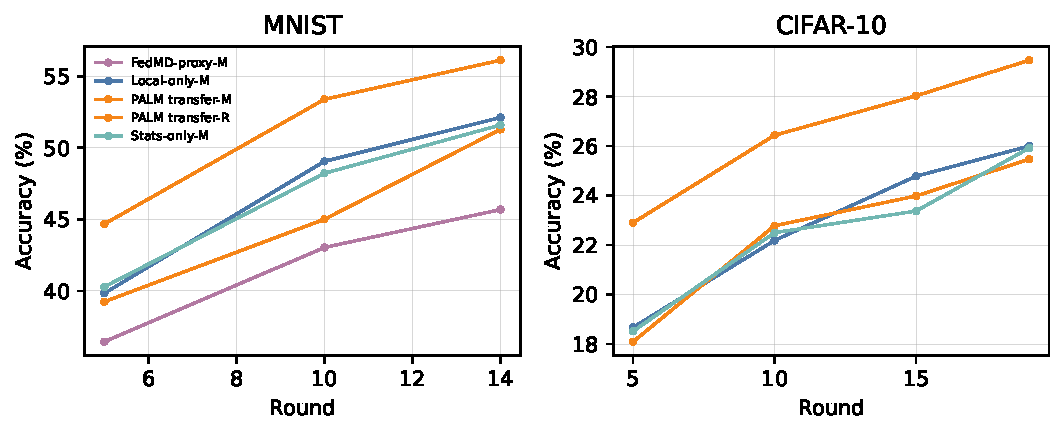
\includegraphics[width=0.96\textwidth]{fig2_learning_curves.pdf}
    \caption{Learning curves from the curated trace-derived independent-split runs. MNIST curves are averaged over seeds 42, 43, and 44; CIFAR-10 curves use the completed trace-calibrated seed-42 case study.}
    \label{fig:learning_curves}
\end{figure*}

\begin{table*}[t]
\centering
\caption{Trace-derived PALM-FL operating comparison. Accuracy is reported in \%. MNIST rows report mean $\pm$ sample standard deviation over three independent repartitions. CIFAR-10 rows report the completed trace-calibrated seed-42 case study.}
\label{tab:main_results}
\begin{threeparttable}
\setlength{\tabcolsep}{3pt}
\scriptsize
\begin{tabular}{llccccccc}
\toprule
Dataset & Mode & \makecell{Acc.\\(\%)} & F1 & \makecell{Up.\\(MB)} & \makecell{Down.\\(MB)} & \makecell{Time\\(s)} & \makecell{Energy\\(J)} & \makecell{Summary\\$\varepsilon_{\max}$} \\
\midrule
MNIST & \localonly & $52.12{\pm}4.21$ & $0.4159{\pm}0.0485$ & 0.0000 & 0.0000 & 16.24 & \best{5.92} & -- \\
MNIST & \statsonly & $51.59{\pm}4.74$ & $0.4104{\pm}0.0526$ & 0.0148 & 0.0000 & 16.25 & 5.98 & 140.69 \\
MNIST & \statstransfer{}-M & $51.29{\pm}3.85$ & $0.4056{\pm}0.0422$ & 0.0148 & 0.0150 & 16.59 & 6.88 & 140.69 \\
MNIST & \statstransfer{}-R & \best{$56.11{\pm}3.99$} & \best{$0.4459{\pm}0.0461$} & 0.0148 & 0.0150 & 23.27 & 6.87 & 100.92 \\
\midrule
CIFAR-10 & \localonly & 26.00 & 0.1589 & 0.0000 & 0.0000 & 58.98 & 10.36 & -- \\
CIFAR-10 & \statsonly & 25.92 & 0.1563 & 0.0197 & 0.0000 & 58.99 & 10.36 & 194.34 \\
CIFAR-10 & \statstransfer{}-M & 25.47 & 0.1487 & 0.0197 & 0.0199 & 59.51 & 10.45 & 194.34 \\
CIFAR-10 & \statstransfer{}-R & \best{29.47} & \best{0.1787} & 0.0197 & 0.0199 & 59.51 & \best{9.82} & 129.58 \\
\bottomrule
\end{tabular}
\begin{tablenotes}[flushleft]
\footnotesize
\item ``M'' and ``R'' denote mobile-aware and random schedulers. Privacy values are client-summary accounting values, not sample-level end-to-end DP certificates. ``--'' means the summary-release accountant is not applicable to that row.
\end{tablenotes}
\end{threeparttable}
\end{table*}

\subsection{Reference baselines}
Table~\ref{tab:baseline_reference} reports the baseline references. FedAvg remains the high-accuracy reference because it assumes a single shared architecture and full-model exchange. On MNIST it reaches $95.98\pm1.35\%$ accuracy but uploads and downloads $1.5996$ MB per selected-client set. Its lower predicted time and energy in this table should not be read as a like-for-like systems win over PALM-FL, because FedAvg uses a homogeneous \texttt{small\_cnn} workload rather than the heterogeneous client models used by PALM-FL. FedProto-style has the same compact payload scale as PALM transfer but lacks the stat-head and contrastive terms. FedMD-style provides a true heterogeneous distillation reference with a public proxy split and $0.0781$ MB proxy-logit upload and downlink on MNIST. It underperforms PALM random transfer in this setting, indicating that proxy-logit exchange alone is not a sufficient replacement for the latent-memory design. CIFAR-10 FedProto-style and FedMD-style trace-derived reruns are not yet complete, so they are omitted rather than mixed with older fixed-split artifacts.

\begin{table*}[t]
\centering
\caption{Trace-derived baseline references. MNIST rows report mean $\pm$ standard deviation over three independent repartitions. The CIFAR-10 FedAvg row reports the completed seed-42 trace case study.}
\label{tab:baseline_reference}
\begin{threeparttable}
\setlength{\tabcolsep}{3pt}
\scriptsize
\begin{tabular}{llccccccc}
\toprule
Dataset & Baseline & \makecell{Acc.\\(\%)} & F1 & \makecell{Up.\\(MB)} & \makecell{Down.\\(MB)} & \makecell{Time\\(s)} & \makecell{Energy\\(J)} & \makecell{Summary\\$\varepsilon_{\max}$} \\
\midrule
MNIST & FedAvg & $95.98{\pm}1.35$ & $0.9594{\pm}0.0137$ & 1.5996 & 1.5996 & 8.30 & 3.46 & -- \\
MNIST & FedProto-style & $50.23{\pm}3.97$ & $0.3959{\pm}0.0436$ & 0.0148 & 0.0150 & 16.25 & 6.89 & 140.69 \\
MNIST & FedMD-style & $45.68{\pm}4.18$ & $0.3436{\pm}0.0524$ & 0.0781 & 0.0781 & 11.96 & 3.55 & -- \\
CIFAR-10 & FedAvg & 59.39 & 0.5464 & 1.7292 & 1.7292 & 13.58 & 9.27 & -- \\
\bottomrule
\end{tabular}
\begin{tablenotes}[flushleft]
\footnotesize
\item ``--'' means the method is not accounted under PALM-FL's clipped summary-release mechanism; it should not be read as a privacy guarantee.
\end{tablenotes}
\end{threeparttable}
\end{table*}

\subsection{Communication, privacy, and fairness}
Figure~\ref{fig:comm_privacy} separates the communication and privacy dimensions for the heterogeneous PALM operating modes. The \statsonly{} mode keeps downlink at zero, while transfer adds a compact prototype package. FedAvg is omitted from this plot because its full-model payload is roughly two orders of magnitude larger and is reported separately in Table~\ref{tab:baseline_reference}. The privacy panel also clarifies that the current $\varepsilon$ values are high: PALM should be read as a clipped-and-noised summary-release mechanism, not as a strong sample-level DP system.

\begin{figure*}[t]
    \centering
    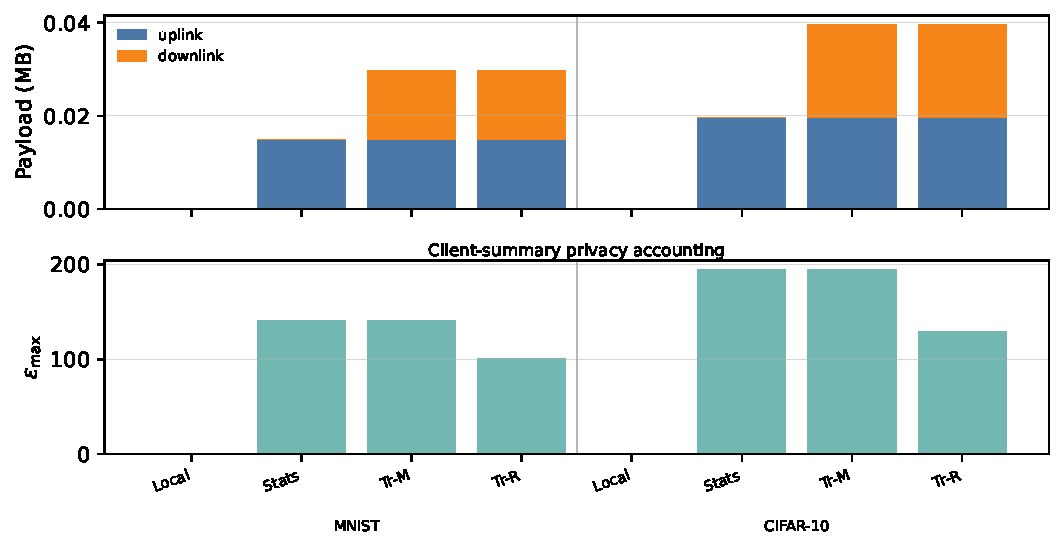
\includegraphics[width=0.96\textwidth]{fig6_comm_privacy_bars.pdf}
\caption{Reported round-level communication and client-summary privacy values from the curated trace-derived runs. \statsonly{} has zero downlink; \statstransfer{} adds a compact masked prototype package.}
    \label{fig:comm_privacy}
\end{figure*}

\begin{figure*}[t]
    \centering
    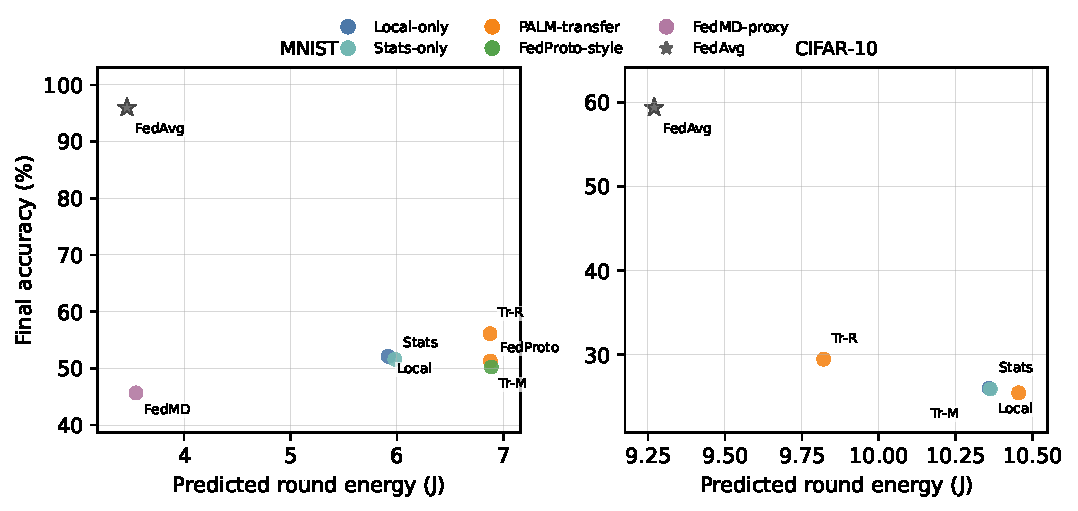
\includegraphics[width=0.88\textwidth]{fig5_accuracy_energy_frontier.pdf}
    \caption{Accuracy--energy operating frontier from the curated trace-derived runs. Each dataset is plotted separately to distinguish heterogeneous PALM-FL operating modes from the homogeneous FedAvg reference.}
    \label{fig:accuracy_energy_frontier}
\end{figure*}

Figure~\ref{fig:arch_fairness} summarizes per-architecture final accuracy for PALM random transfer. The architecture-level spread is substantial, especially on CIFAR-10, which shows why heterogeneous-FL papers should report client-group behavior rather than only averaged endpoint accuracy. In the MNIST three-seed run, \texttt{tiny\_resnet} clients benefit most from the random-transfer operating point, while \texttt{wide\_cnn} clients remain weaker under the non-IID splits used here.

\begin{figure*}[t]
    \centering
    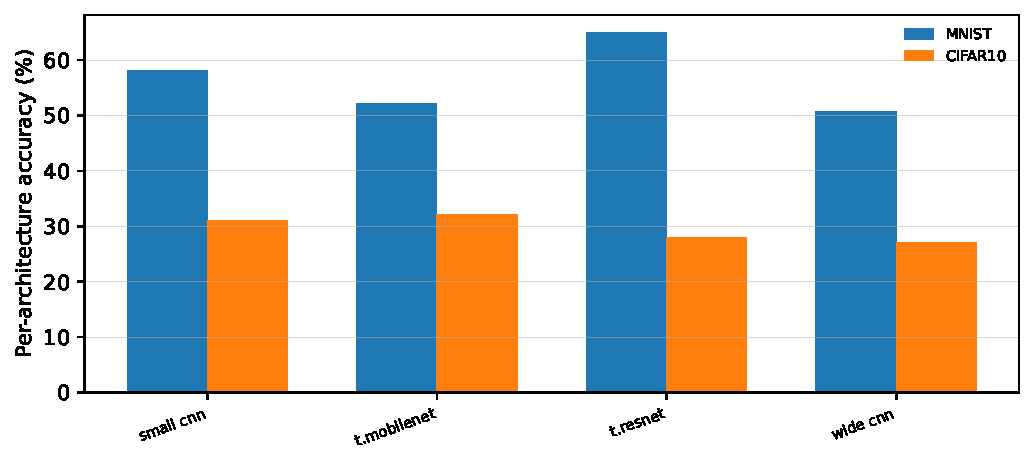
\includegraphics[width=0.90\textwidth]{fig7_architecture_fairness.pdf}
    \caption{Per-architecture final accuracy for PALM random transfer. MNIST bars aggregate three independent repartitions; CIFAR-10 bars use the completed seed-42 trace case study.}
    \label{fig:arch_fairness}
\end{figure*}

\subsection{Discussion}
Four points follow directly from the evidence. First, upload-only \statsonly{} remains the safest low-communication operating mode because it tracks \localonly{} while keeping downlink at zero; it does not demonstrate a strong federated learning gain. Second, transfer helps most when the scheduler provides broader client and class coverage; random participation improves MNIST and CIFAR-10 seed-42 utility, whereas mobile-aware transfer stays near the lower-cost local/statistics operating point. Third, FedAvg confirms the accuracy available when the problem is changed to homogeneous full-model sharing, but it is not a like-for-like heterogeneous systems comparison. Fourth, the trace-derived profile changes the cost scale relative to a synthetic profile, so claims based only on uniformly sampled bandwidth would be misleading.

Table~\ref{tab:generated_ablation_status} reports completed MNIST and CIFAR-10 ablations over seeds 42, 43, and 44. The histogram-only rows are important because they show that clipped-and-noised class counts alone can produce competitive utility under random participation. The mean-only rows are also diagnostic, but they use noisy availability rather than the full count-deficit signal. The no-noise rows are explicitly non-private diagnostics, and the count-only transfer row removes prototype vectors from the downlink package. These rows improve claim isolation, but they do not prove that latent moments are the dominant source of utility: on CIFAR-10, random histogram-only and random mean-only are close, and no-deficit random transfer remains close to the original random-transfer case-study endpoint.

\begin{table*}[t]
\centering
\caption{Ablation study isolating count, latent, noise, transfer, and scheduler effects. Completed MNIST and CIFAR-10 ablation rows use seeds 42, 43, and 44.}
\label{tab:generated_ablation_status}
\scriptsize
\resizebox{\textwidth}{!}{%
\begin{tabular}{lllllllllll}
\toprule
Dataset & Mode & Scheduler & Accuracy & Macro-F1 & Upload MB & Download MB & Predicted time s & Predicted energy J & Epsilon/accounting & Interpretation \\
\midrule
MNIST & histogram-only & mobile & 48.96$\pm$5.09 & 0.3858$\pm$0.0485 & 0.0002 & 0.0000 & 11.55 & 3.34 & 61.70 & counts-only scheduler control; three MNIST seeds \\
MNIST & histogram-only & random & 56.51$\pm$3.46 & 0.4527$\pm$0.0391 & 0.0002 & 0.0000 & 22.77 & 6.73 & 45.58 & counts-only random-participation control; three MNIST seeds \\
MNIST & mean-only & mobile & 50.80$\pm$2.76 & 0.4064$\pm$0.0315 & 0.0075 & 0.0000 & 16.25 & 5.92 & 102.88 & latent means with noisy availability; three MNIST seeds \\
MNIST & mean-only & random & 55.70$\pm$4.24 & 0.4449$\pm$0.0536 & 0.0075 & 0.0000 & 22.77 & 6.73 & 74.61 & latent means under random participation; three MNIST seeds \\
MNIST & stats-only no-noise & mobile & 51.32$\pm$5.10 & 0.4060$\pm$0.0552 & 0.0148 & 0.0000 & 16.25 & 5.98 & non-private diagnostic & non-private summary diagnostic; three MNIST seeds \\
MNIST & transfer no-noise & mobile & 52.17$\pm$2.89 & 0.4163$\pm$0.0332 & 0.0148 & 0.0150 & 17.96 & 4.48 & non-private diagnostic & non-private transfer diagnostic; three MNIST seeds \\
MNIST & count-only transfer & mobile & 52.09$\pm$2.84 & 0.4129$\pm$0.0421 & 0.0002 & 0.0003 & 20.88 & 4.87 & 61.70 & transfer package without prototypes; three MNIST seeds \\
MNIST & Stats-only & mobile/no\_deficit & 51.02$\pm$4.09 & 0.4056$\pm$0.0466 & 0.0148 & 0.0000 & 16.25 & 5.92 & 140.69 & full-summary scheduler without released-count deficit; three MNIST seeds \\
MNIST & stats-transfer-M & mobile/no\_deficit & 50.55$\pm$3.47 & 0.4023$\pm$0.0403 & 0.0148 & 0.0150 & 16.59 & 6.01 & 140.69 & mobile transfer without released-count deficit; three MNIST seeds \\
MNIST & stats-transfer-R & random/no\_deficit & 55.49$\pm$3.93 & 0.4426$\pm$0.0450 & 0.0148 & 0.0150 & 23.27 & 6.87 & 100.92 & random transfer without released-count deficit; three MNIST seeds \\
CIFAR-10 & histogram-only & mobile & 26.96$\pm$2.52 & 0.1738$\pm$0.0281 & 0.0002 & 0.0000 & 38.50 & 12.63 & 81.89 & counts-only scheduler control; three CIFAR-10 seeds \\
CIFAR-10 & histogram-only & random & 32.28$\pm$2.59 & 0.2132$\pm$0.0270 & 0.0002 & 0.0000 & 79.12 & 19.10 & 56.07 & counts-only random-participation control; three CIFAR-10 seeds \\
CIFAR-10 & mean-only & mobile & 28.56$\pm$3.19 & 0.1861$\pm$0.0323 & 0.0100 & 0.0000 & 41.09 & 16.29 & 138.85 & latent means with noisy availability; three CIFAR-10 seeds \\
CIFAR-10 & mean-only & random & 32.73$\pm$2.25 & 0.2163$\pm$0.0211 & 0.0100 & 0.0000 & 79.13 & 19.11 & 92.96 & latent means under random participation; three CIFAR-10 seeds \\
CIFAR-10 & stats-only no-noise & mobile & 28.33$\pm$1.73 & 0.1860$\pm$0.0208 & 0.0197 & 0.0000 & 41.09 & 16.30 & non-private diagnostic & non-private summary diagnostic; three CIFAR-10 seeds \\
CIFAR-10 & transfer no-noise & mobile & 28.20$\pm$1.86 & 0.1800$\pm$0.0237 & 0.0197 & 0.0199 & 41.45 & 16.44 & non-private diagnostic & non-private transfer diagnostic; three CIFAR-10 seeds \\
CIFAR-10 & count-only transfer & mobile & 28.73$\pm$2.45 & 0.1876$\pm$0.0275 & 0.0002 & 0.0003 & 41.44 & 16.43 & 81.89 & transfer package without prototypes; three CIFAR-10 seeds \\
CIFAR-10 & Stats-only & mobile/no\_deficit & 28.73$\pm$2.45 & 0.1876$\pm$0.0275 & 0.0197 & 0.0000 & 41.09 & 16.30 & 191.71 & full-summary scheduler without released-count deficit; three CIFAR-10 seeds \\
CIFAR-10 & stats-transfer-M & mobile/no\_deficit & 28.48$\pm$2.64 & 0.1811$\pm$0.0281 & 0.0197 & 0.0199 & 41.45 & 16.44 & 191.71 & mobile transfer without released-count deficit; three CIFAR-10 seeds \\
CIFAR-10 & stats-transfer-R & random/no\_deficit & 32.82$\pm$3.17 & 0.2133$\pm$0.0305 & 0.0197 & 0.0199 & 79.83 & 19.28 & 126.69 & random transfer without released-count deficit; three CIFAR-10 seeds \\
\bottomrule
\end{tabular}
}
\end{table*}


\section{Limitations and Future Work}
The mobile validation is trace-derived for bandwidth only; real-device training latency and battery power measurements remain necessary for deployment claims. The time and energy values should therefore be interpreted as operating estimates from a cost model, not as measured phone energy. The MNIST main table uses independent repartitions, but the primary CIFAR-10 operating-mode and baseline comparison still has only a completed seed-42 trace case study, so a full three- or five-seed CIFAR-10 trace rerun is needed for stable main-result claims. The present study also uses ten clients and two image datasets; larger cross-device populations and additional mobile workloads are needed. The privacy accountant is participation-counted zCDP over clipped client summaries and does not certify end-to-end sample-level DP. The $\varepsilon$ values are high, and full-model/proxy-logit baselines are not DP-accounted, so the claim should remain limited to privacy-scoped summary release. The new ablations in Table~\ref{tab:generated_ablation_status} are three-seed diagnostics on both datasets, but they show that counts, participation coverage, and scheduler choice explain much of the observed behavior; therefore, the value of latent moments beyond clipped-and-noised class-count balancing remains only partially isolated. Finally, FedAvg, FedProto-style, and FedMD-style references improve baseline coverage, but reproducing stronger submodel and distillation baselines such as HeteroFL/FjORD, NeFL, GEFL/GEFL-F, and FedDF/FedGH would further strengthen the empirical comparison.

\section{Conclusion}
PALM-FL addresses heterogeneous mobile federated learning through clipped-and-noised client-summary release and resource-aware client selection. The framework avoids architecture-specific parameter aggregation, sanitizes compact class-wise summaries before upload, and makes participation decisions under explicit communication, time, and energy budgets. The experiments use independent MNIST repartitions and public trace-derived mobile bandwidth profiles. The results show that \statsonly{} preserves the low-payload local-training operating point, while masked \statstransfer{} can improve utility when scheduler coverage is broad enough. PALM-FL is therefore best positioned as an architecture-flexible, low-payload, privacy-scoped coordination mechanism that complements, rather than replaces, high-accuracy homogeneous full-model FL.

\appendices
\section{Prototype-Transfer Variants}
For completeness, the prototype-transfer family augments \eqref{eq:local_loss} with prototype alignment and prototype cross-entropy terms:
\begin{equation}
\mathcal{L}_k^{\mathrm{proto}} =
\mathcal{L}_k + \lambda_a\mathcal{L}_{\mathrm{align}}
+ \lambda_p\mathcal{L}_{\mathrm{pCE}}.
\end{equation}
The unmasked prototype-broadcast ablation was useful for controlled comparison but underperformed in the retained experiments. The \statstransfer{} path used in this paper differs by masking unavailable classes and using the prototype bank as a contrastive anchor set.

\begin{thebibliography}{99}

\bibitem{gefl}
H. Kang, S. Cha, and J. Kang, ``GeFL: Model-agnostic federated learning with generative models,'' \emph{IEEE Trans. Mobile Comput.}, vol.~25, no.~4, pp.~4493--4505, Apr.~2026, doi: 10.1109/TMC.2025.3592483.

\bibitem{mobilebandwidth}
X. Yang \emph{et al.}, ``Mobile access bandwidth in practice: Measurement, analysis, and implications,'' in \emph{Proc. ACM SIGCOMM}, 2022, pp.~114--128, doi: 10.1145/3544216.3544237.

\bibitem{fedavg}
B. McMahan, E. Moore, D. Ramage, S. Hampson, and B. A. y Arcas, ``Communication-efficient learning of deep networks from decentralized data,'' in \emph{Proc. AISTATS}, 2017, pp.~1273--1282.

\bibitem{fedprox}
T. Li, A. K. Sahu, M. Zaheer, M. Sanjabi, A. Talwalkar, and V. Smith, ``Federated optimization in heterogeneous networks,'' in \emph{Proc. MLSys}, 2020, pp.~429--450.

\bibitem{scaffold}
S. P. Karimireddy, S. Kale, M. Mohri, S. Reddi, S. Stich, and A. T. Suresh, ``SCAFFOLD: Stochastic controlled averaging for federated learning,'' in \emph{Proc. ICML}, 2020, pp.~5132--5143.

\bibitem{fedala}
J. Zhang \emph{et al.}, ``FedALA: Adaptive local aggregation for personalized federated learning,'' in \emph{Proc. AAAI}, 2023, pp.~11237--11244.

\bibitem{pfeiffer}
K. Pfeiffer, M. Rapp, R. Khalili, and J. Henkel, ``Federated learning for computationally constrained heterogeneous devices: A survey,'' \emph{ACM Comput. Surv.}, vol.~55, no.~14s, pp.~1--27, Jul.~2023.

\bibitem{nguyen}
D. C. Nguyen, M. Ding, P. N. Pathirana, A. Seneviratne, J. Li, and H. V. Poor, ``Federated learning for Internet of Things: A comprehensive survey,'' \emph{IEEE Commun. Surv. Tuts.}, vol.~23, no.~3, pp.~1622--1658, 2021.

\bibitem{nefl}
H. Kang, S. Cha, J. Shin, J. Lee, and J. Kang, ``NeFL: Nested model scaling for federated learning with system heterogeneous clients,'' \emph{IEEE Trans. Mobile Comput.}, vol.~24, no.~8, pp.~6734--6746, Aug.~2025.

\bibitem{avgkd}
A. Afonin and S. P. Karimireddy, ``Towards model agnostic federated learning using knowledge distillation,'' in \emph{Proc. ICLR}, 2022.

\bibitem{fjord}
S. Horv\'ath, S. Laskaridis, M. Almeida, I. Leontiadis, S. Venieris, and N. Lane, ``FjORD: Fair and accurate federated learning under heterogeneous targets with Ordered Dropout,'' in \emph{Proc. NeurIPS}, 2021, pp.~12876--12889.

\bibitem{depthfl}
M. Kim, S. Yu, S. Kim, and S.-M. Moon, ``DepthFL: Depthwise federated learning for heterogeneous clients,'' in \emph{Proc. ICLR}, 2023.

\bibitem{heterofl}
E. Diao, J. Ding, and V. Tarokh, ``HeteroFL: Computation and communication efficient federated learning for heterogeneous clients,'' in \emph{Proc. ICLR}, 2021.

\bibitem{feddf}
T. Lin, L. Kong, S. U. Stich, and M. Jaggi, ``Ensemble distillation for robust model fusion in federated learning,'' in \emph{Proc. NeurIPS}, 2020, pp.~2351--2363.

\bibitem{fccl}
W. Huang, M. Ye, and B. Du, ``Learn from others and be yourself in heterogeneous federated learning,'' in \emph{Proc. CVPR}, 2022, pp.~10133--10143.

\bibitem{fedmd}
D. Li and J. Wang, ``FedMD: Heterogenous federated learning via model distillation,'' arXiv:1910.03581, 2019.

\bibitem{fedgh}
L. Yi, G. Wang, X. Liu, Z. Shi, and H. Yu, ``FedGH: Heterogeneous federated learning with generalized global header,'' arXiv:2303.13137, 2023.

\bibitem{fedproto}
Y. Tan \emph{et al.}, ``FedProto: Federated prototype learning across heterogeneous clients,'' in \emph{Proc. AAAI}, 2022, pp.~8432--8440.

\bibitem{lgfedavg}
P. P. Liang, T. Liu, L. Ziyin, R. Salakhutdinov, and L.-P. Morency, ``Think locally, act globally: Federated learning with local and global representations,'' arXiv:2001.01523, 2020.

\bibitem{fml}
T. Shen \emph{et al.}, ``Federated mutual learning,'' arXiv:2006.16765, 2020.

\bibitem{pfedhr}
J. Wang \emph{et al.}, ``Towards personalized federated learning via heterogeneous model reassembly,'' arXiv:2308.08643, 2023.

\bibitem{fedgan}
M. Rasouli, T. Sun, and R. Rajagopal, ``FedGAN: Federated generative adversarial networks for distributed data,'' arXiv:2006.07228, 2020.

\bibitem{fedcg}
Y. Wu, Y. Kang, J. Luo, Y. He, and Q. Yang, ``FedCG: Leverage conditional GAN for protecting privacy and maintaining competitive performance in federated learning,'' arXiv:2111.08211, 2021.

\bibitem{datafreekd}
Z. Zhu, J. Hong, and J. Zhou, ``Data-free knowledge distillation for heterogeneous federated learning,'' in \emph{Proc. ICML}, 2021, pp.~12878--12889.

\bibitem{finetunekd}
L. Zhang, L. Shen, L. Ding, D. Tao, and L. Duan, ``Fine-tuning global model via data-free knowledge distillation for non-IID federated learning,'' in \emph{Proc. CVPR}, 2022, pp.~10164--10173.

\bibitem{fedclassavg}
J. Jang, H. Ha, D. Jung, and S. Yoon, ``FedClassAvg: Local representation learning for personalized federated learning on heterogeneous neural networks,'' in \emph{Proc. ICPP}, 2022, pp.~1--10.

\bibitem{mori}
J. Mori, I. Teranishi, and R. Furukawa, ``Continual horizontal federated learning for heterogeneous data,'' in \emph{Proc. IJCNN}, 2022, pp.~1--8.

\bibitem{mnist}
Y. LeCun, L. Bottou, Y. Bengio, and P. Haffner, ``Gradient-based learning applied to document recognition,'' \emph{Proc. IEEE}, vol.~86, no.~11, pp.~2278--2324, Nov.~1998.

\bibitem{cifar10}
A. Krizhevsky, V. Nair, and G. Hinton, ``Learning multiple layers of features from tiny images,'' Master's thesis, Dept. Comput. Sci., Univ. Toronto, Toronto, ON, Canada, 2009.

\bibitem{abadi}
M. Abadi \emph{et al.}, ``Deep learning with differential privacy,'' in \emph{Proc. ACM CCS}, 2016, pp.~308--318.

\bibitem{zcdp}
M. Bun and T. Steinke, ``Concentrated differential privacy: Simplifications, extensions, and lower bounds,'' in \emph{Proc. TCC}, 2016, pp.~635--658.

\bibitem{dpgan}
L. Xie, K. Lin, S. Wang, F. Wang, and J. Zhou, ``Differentially private generative adversarial network,'' arXiv:1802.06739, 2018.

\bibitem{zeiler}
M. D. Zeiler and R. Fergus, ``Visualizing and understanding convolutional networks,'' in \emph{Proc. ECCV}, 2014, pp.~818--833.

\bibitem{mahendran}
A. Mahendran and A. Vedaldi, ``Understanding deep image representations by inverting them,'' in \emph{Proc. CVPR}, 2015, pp.~5188--5196.

\bibitem{dosovitskiy}
A. Dosovitskiy and T. Brox, ``Inverting visual representations with convolutional networks,'' in \emph{Proc. CVPR}, 2016, pp.~4829--4837.

\bibitem{bladefl}
J. Li \emph{et al.}, ``Blockchain assisted decentralized federated learning (BLADE-FL): Performance analysis and resource allocation,'' \emph{IEEE Trans. Parallel Distrib. Syst.}, vol.~33, no.~10, pp.~2401--2415, Oct.~2022.

\end{thebibliography}

\end{document}
